\chapter{BACKUP: Validation in liquid jet in crossflow}
	\label{ch6:jicf_lgs_simulations}

\section{(OLD) Numerical experiments (OLD)}

\hl{ALSO: effect of one and two-way coupling !! Ver articulos 2010, 2011 Li }.

%
\begin{figure}[h!]	
	\centering
	\includeinkscape[inkscapelatex=false,scale=0.3]{./part2_developments/figures_ch6_lagrangian_JICF/chart_input_parameters_LGS}
	\caption{Parameters tested}\label{fig:BACKUP_dispersed_phase_sli_parameters}
\end{figure}


\subsection{Design of experiments}

In Chapter \ref{ch5:jicf_resolved_simulations}, the five resolved atomization simulations from Table \ref{fig:location_JICF_ops_in_breakup_map} were performed and analyzed. These ones tested two mesh interface mesh resolutions ($\Delta x_\mathrm{min} = 20, 10~\mu$m), two operating points ($We_g = 830, 1470$) and the influence of turbulence injection in one simulation for the coarse resolution, high $We_g$ case. Results shown a high dependency of the trajectories ($\S$\ref{subsec:ch5_jet_trajectories_results}) and jet topologies ($\S$\ref{sec:ch5_jet_evolution}) on the resolution, which led later to different spray characteristics ($\S$\ref{sec:ch5_sec_spray_characterization}) and resulting injectors ($\S$\ref{sec:ch5_learning_SLI}) for each case, which a high dependency on the operating point due to the different velocity magnitudes involved. Therefore, it is of interest to test such effects in the disperse-phase simulations by initializing these computations with the different injectors obtained.

Apart from the resolved simulation parameters (i.e. $\Delta x_\mathrm{min}$, operating condition, turbulence injection), the SLI parameters to perform injection derived in Chapter \ref{ch4:sli_development} and summarized in Table \ref{subsec:ch4_injectors_definition} can also be tested, as well as the influence of the ALM model ($\S$\ref{sec:ch4_dense_core_modelling}) and the secondary atomization models ($\S$\ref{sec:ch4_dense_core_modelling}). The influence of all these parameters can be studied by performing a design of experiments with consists of the simulations from Table \ref{tab:lgs_jicf_DoF}, and which proceeds as follows: 


\begin{itemize}

	\item A \textbf{baseline} case is selected to perform injection. The resolved case UG100\_DX10 is chosen with injection being performed at $x_\mathrm{inj} = 5$ mm, ALM activated, Gaussian $\textbf{r}$  law and Gorokhovski's atomization model ($\S$\ref{subsec:ch4_goro_model}). \hl{This case was studied in ... and has been selected because ...}. It corresponds to case 1 from Table \ref{tab:lgs_jicf_DoF}, and all the rest of dispersed-phase simulations are compared to this case.

		\item The effect of the \textbf{resolved mesh resolution} in the injectors is studied by keeping all parameters identical but choosing the SLI obtained from case UG100\_DX20 (see Figure \textbf{XX}). It corresponds to case 2 from Table \ref{tab:lgs_jicf_DoF}

	\item The effect of \textbf{injection location} $x_\mathrm{inj}$ downstream the injector nozzle. The resolved JICF trajectories from Figure \ref{fig:JICF_trajectories_validation} show that the numerical trajectories are properly estimated in the near-nozzle region but that after a certain point, the coarse resolutions underestimate the trajectory while the fine ones overestimate it. To study the influence this can have in the dispesed-phase simulations, three different simulations are performed: two simulations for the resolved case UG100\_DX10 at 1) $x = 5$ mm ($x/d_\mathrm{inj} = 11$);, where the trajectory is properly estimated, and 2) $x = 10$ mm ($x/d_\mathrm{inj} = 22$) where the trajectory is overestimated; and 3) one simulation for the resolved case UG100\_DX20 at $x = 10$ mm ($x/d_\mathrm{inj} = 22$), where the trajectory is underestimated. These cases have been considered since they present low relative values for mass conservation of liquid mass, as shown in Figure \ref{fig:delta_Ql_with_x}. Both simulations performed correspond to cases 3 and 4 from Table \ref{tab:lgs_jicf_DoF}.
	
	\item The \textbf{operating condition} is tested by simulating the case UG75\_DX10 with the rest of parameters identical to the baseline (case 5 from Table \ref{tab:lgs_jicf_DoF}).
	
	\item \hl{The effect of the \textbf{injection diameters law} $f_0$ ...}
	
	\item \textbf{Spray velocities in the SLI} are tested by simulating the baseline case with the two other $\text{r}$ laws: uniform and zero, corresponding to cases 6 and 7 from Table \ref{tab:lgs_jicf_DoF}.
	
	\item A simulation without \textbf{ALM} is performed (case 8 from Table \ref{tab:lgs_jicf_DoF}).
	
	\item Finally, the effect of the different atomization models is tested by using the TAB and ETAB modes with the baseline conditions (cases 9 and 10 from Table \ref{tab:lgs_jicf_DoF}).	
	
\end{itemize}

\clearpage
	
%\begin{table}[!h]
%\centering
%\caption{Design of experiments to test injection parameters. Modified parameters are highlighted in blue.}
%\begin{tabular}{ccccccc}
%\thickhline
%\multirow{2}{*}{ \textbf{Case}} &  \multirow{2}{*}{ \begin{tabular}{c} \textbf{Resolved} \\ \textbf{simulation} \end{tabular}}    &  \multirow{2}{*}{  \begin{tabular}{c} $x_\mathrm{inj}$  \\ $\left[ \mathrm{mm} \right]$ \end{tabular}} &   \multirow{2}{*}{ \begin{tabular}{c} $\textbf{r}$ \\ \textbf{law} \end{tabular}} & \multirow{2}{*}{ \textbf{ALM ?}}  & \multirow{2}{*}{ \begin{tabular}{c} \textbf{Atomization} \\ \textbf{model} \end{tabular}} &    \multirow{2}{*}{ \textbf{Description}}\\
% & & & & & & \\
%\thickhline
%\vspace*{0.1in}
%1 & UG100\_DX10 & 5 & Gaussian & Yes & Goro  & Baseline \tab_space
%\multirow{2}{*}{2} & \multirow{2}{*}{UG100\_\textcolor{blue}{DX20}} & \multirow{2}{*}{5} & \multirow{2}{*}{Gaussian} & \multirow{2}{*}{Yes} & \multirow{2}{*}{Goro}  &  
% \multirow{2}{*}{ \begin{tabular}{c} Effect of \\ resolution \end{tabular}} \\
% & & & & & & \tab_space
%3 & UG100\_DX10 & \textcolor{blue}{10} & Gaussian & Yes & Goro  & Effect of $x_\mathrm{inj}$ \tab_space
%4 & UG100\_\textcolor{blue}{DX20} & \textcolor{blue}{10} & Gaussian & Yes & Goro  & Effect of $x_\mathrm{inj}$ \tab_space
%\multirow{2}{*}{5} & \multirow{2}{*}{\textcolor{blue}{UG75}\_DX10} & \multirow{2}{*}{10} & \multirow{2}{*}{Gaussian} & \multirow{2}{*}{Yes} & \multirow{2}{*}{Goro}  & \multirow{2}{*}{ \begin{tabular}{c} Effect of  \\ operating condition  \end{tabular}} \\
% & & & & & & \tab_space
%6 & UG100\_DX10 & 5 & \textcolor{blue}{Uniform} & Yes & Goro  & Effect of $r$ law \tab_space
%7 & UG100\_DX10 & 5 & \textcolor{blue}{Zero} & Yes & Goro  & Effect of $r$ law \tab_space
%8 & UG100\_DX10 & 5 & Gaussian & \textcolor{blue}{No} & Goro  & Effect of ALM \tab_space
%\multirow{2}{*}{9} & \multirow{2}{*}{UG100\_DX10} & \multirow{2}{*}{5} & \multirow{2}{*}{Gaussian} & \multirow{2}{*}{Yes} & \multirow{2}{*}{\textcolor{blue}{TAB}} & \multirow{2}{*}{ \begin{tabular}{c} Effect of  \\ atomization model\end{tabular}}\\
% & & & & & & \tab_space
%\multirow{2}{*}{10} & \multirow{2}{*}{UG100\_DX10} & \multirow{2}{*}{5} & \multirow{2}{*}{Gaussian} & \multirow{2}{*}{Yes} & \multirow{2}{*}{\textcolor{blue}{ETAB}} & \multirow{2}{*}{ \begin{tabular}{c} Effect of  \\ atomization model\end{tabular}}\\
% & & & & & & \tab_space
%\thickhline
%\end{tabular}
%\label{tab:lgs_jicf_DoF}
%\end{table}

	
\begin{table}[!h]
\centering
\caption{Design of experiments to test injection parameters. Blue highlight indicates modified parameters.}
\begin{tabular}{ccccccc}
\thickhline
\multirow{2}{*}{ \textbf{Case}} &  \multirow{2}{*}{ \begin{tabular}{c} \textbf{Resolved} \\ \textbf{simulation} \end{tabular}}    &  \multirow{2}{*}{  \begin{tabular}{c} $x_\mathrm{inj}$  \\ $\left[ \mathrm{mm} \right]$ \end{tabular}} &   \multirow{2}{*}{ \begin{tabular}{c} $\textbf{r}$ \\ \textbf{law} \end{tabular}} & \multirow{2}{*}{ \textbf{ALM ?}}  & \multirow{2}{*}{ \begin{tabular}{c} \textbf{Atomization} \\ \textbf{model} \end{tabular}} &    \multirow{2}{*}{ \textbf{Modification}}\\
 & & & & & & \\
\thickhline
1 & UG100\_DX10 & 5 & Gaussian & Yes & Goro  & Baseline \tab_space
2 & UG100\_\textcolor{blue}{DX20} & 5 & Gaussian & Yes & Goro  & SPS resolution \tab_space
3 & UG100\_DX10 & \textcolor{blue}{10} & Gaussian & Yes & Goro  & $x_\mathrm{inj}$ \tab_space
4 & UG100\_\textcolor{blue}{DX20} & \textcolor{blue}{10} & Gaussian & Yes & Goro  & $x_\mathrm{inj}$ \tab_space
5 & \textcolor{blue}{UG75}\_DX10 & 10 & Gaussian & Yes & Goro  & Operating condition \tab_space
6 & UG100\_DX10 & 5 & \textcolor{blue}{Uniform} & Yes & Goro  & $r$ law \tab_space
7 & UG100\_DX10 & 5 & \textcolor{blue}{Zero} & Yes & Goro  & $r$ law \tab_space
8 & UG100\_DX10 & 5 & Gaussian & \textcolor{blue}{No} & Goro  & ALM \tab_space
9 & UG100\_DX10 & 5 & Gaussian & Yes & \textcolor{blue}{TAB} & Atomization model \tab_space
10 & UG100\_DX10 & 5 & Gaussian & Yes & \textcolor{blue}{ETAB} & Atomization model \tab_space
\thickhline
\end{tabular}
\label{tab:lgs_jicf_DoF_OLD}
\end{table}

	
\subsection{Results}


\subsubsection*{Effect of mesh resolution}

\subsubsection*{Effect of injection location}

\subsubsection*{Effect of operating condition}

\subsubsection*{Effect of $\textbf{r}$ law}

\subsubsection*{Effect of ALM}

\subsubsection*{Effect of atomization model}

\clearpage

\section{Calibration of secondary atomization model}

\subsection{Apte}

\subsection{Stuff on relative velocities}

OJO: ver pilotage 2021-05-26 para graficas de interes.

\begin{equation}
\overline{\textbf{u}}_\mathrm{rel,SPS} = \overline{\textbf{u}}_{g,\mathrm{SPS}} - \overline{\textbf{u}}_l ~~~~ ; ~~~~  \overline{\textbf{u}}_\mathrm{rel,ALM} = \overline{\textbf{u}}_{g,\mathrm{ALM}} - \overline{\textbf{u}}_l
\end{equation}

\begin{equation}
\Delta u_\mathrm{rel} = | \overline{\textbf{u}}_\mathrm{rel,ALM}| - |\overline{\textbf{u}}_\mathrm{rel,SPS}|
\end{equation}

\begin{equation}
\varepsilon =  \frac{|\overline{\textbf{u}}_\mathrm{rel,ALM}| - |\overline{\textbf{u}}_\mathrm{rel,SPS}|}{|\overline{\textbf{u}}_\mathrm{rel,SPS}|} 
\end{equation}

\begin{equation}
\overline{\textbf{u}}_\mathrm{l,LGS} = \overline{\textbf{u}}_{g,\mathrm{LGS}} - \overline{\textbf{u}}_\mathrm{rel,SPS}
\end{equation}

Modification in secondary breakup:

\begin{equation}
\Delta \textbf{u}_\mathrm{rel} = \textbf{u}_\mathrm{rel,LGS} - \textbf{u}_\mathrm{rel,SPS}
\end{equation}

\begin{equation}
\frac{\Delta \textbf{u}_\mathrm{rel}}{\textbf{u}_\mathrm{rel,SPS}} < \alpha 
\end{equation}


\section{Dispersed phase simulations}


\subsection{Design of experiments}


In Chapter \ref{ch5:jicf_resolved_simulations}, the five resolved atomization simulations from Table \ref{fig:location_JICF_ops_in_breakup_map} were performed and analyzed. These ones tested two mesh interface mesh resolutions ($\Delta x_\mathrm{min} = 20, 10~\mu$m), two operating points ($We_g = 830, 1470$) and the influence of turbulence injection in one simulation for the coarse resolution, high $We_g$ case. Results shown a high dependency of the trajectories ($\S$\ref{subsec:ch5_jet_trajectories_results}) and jet topologies ($\S$\ref{sec:ch5_jet_evolution}) on the resolution, which led later to different spray characteristics ($\S$\ref{sec:ch5_sec_spray_characterization}) and resulting injectors ($\S$\ref{sec:ch5_learning_SLI}) for each case, which a high dependency on the operating point due to the different velocity magnitudes involved. Therefore, it is of interest to test such effects in the disperse-phase simulations by initializing these computations with the different injectors obtained.

Apart from the different injectors obtained from the resolved simulations (i.e. $\Delta x_\mathrm{min}$, operating condition, turbulence injection), the SLI parameters to perform injection derived in Chapter \ref{ch4:sli_development} and summarized in Table \ref{subsec:ch4_injectors_definition} are tested, as well as the influence of the ALM model ($\S$\ref{sec:ch4_dense_core_modelling}) and the secondary atomization models ($\S$\ref{sec:ch4_dense_core_modelling}). Figure \ref{fig:dispersed_phase_sli_parameters} shows the different models involved in the dispersed phase simulations with their control parameters: they are split into the possible influences on the gas and liquid phases, as well as the secondary breakup which is considered as an interaction between both (even though it acts on the liquid phase, it needs the gas velocity for calculating the relative velocity in order to estimate liquid brekaup). The influence of all these parameters can be studied by performing a Design of Experiments (DoE) where each relevant parameter is assessed individually. Due to the large number of parameters, \hl{four} different sets of simulations (summarized in Table \ref{tab:lgs_jicf_DoF}) are performed and validated with the experimental results:

\begin{itemize}

	\item \textbf{Set I}: the effect of the gaseous phase boundary conditions is checked in first place. According to the parameters shown in Figure \ref{fig:dispersed_phase_sli_parameters} and the results from $\S$\ref{sec:ch6_BC_gaseous_phase}, \hl{four} simulations are performed to test the: 1) unperturbed case, 2) perturbed case with baseline ALM, 3) perturbed case with optimum ALM, and 4) perturbed case with prescribed inlet. The same SLI is used for all simulations, which is described in first place. From these simulations, the case \hl{??} has been found to yield the best experimental comparison, and so has been chosen to proceed with the numerical experiments of the set 2.
	
	\item \textbf{Set II}: assessing the effect of the SLI parameters (liquid phase in in Figure \ref{fig:dispersed_phase_sli_parameters}). Parameters tested include the liquid injection velocity law $r$ and the use of convergence-driven discretization to build SLI. \hl{From these simulations, it has been found ...}
	
	\item \textbf{Set III}: effect of the secondary atomization model. The three implemented models (TAB, ETAB and Gorokhovski) are tested. \hl{Two extra parameters}, $\Delta x_\mathrm{atom}$ and $\Delta u_\mathrm{rel}$, ...
	
	\item \textbf{Set IV}: influence of resolved atomization parameters. From the previous analyses, the best configuration is chosen and applied to study the effect of injection location ($x = $10 mm), resolution ($\Delta x_\mathrm{min} = 20~\mu$m), \hl{synthethic turbulence injection in the gaseous inlet} and operating condition (SLI from low Weber operating point.)

\end{itemize}

\clearpage

\begin{table}[!h]
\centering
\caption{Design of experiments to test injection parameters}
\begin{tabular}{ccc}
\thickhline
\textbf{Series} & \textbf{Case} & \textbf{Modification} \\
\thickhline
\multirow{4}{*}{ 1} & 1.1 & No perturbed gaseous inlet \\
& 1.2 & Baseline ALM \\
& 1.3 & Optimum ALM \\
& 1.4 & Prescribed inlet \\
\hline
\multirow{3}{*}{ 2} & 2.1 & $r$ law: uniform \\
& 2.2 & $r$ law: zero \\
& 2.3 & SLI built with convergence-driven discretization \\
\hline
\multirow{2}{*}{ 2} & 3.1 & Atomization model: TAB \\
& 3.2 & Atomization model: TAB \\
\hline
\multirow{4}{*}{ 4} & 4.1 & Injection location: $x_\mathrm{inj} = 10$ mm \\
& 4.2 & Resolution: $\Delta x_\mathrm{min} = 20~\mu$m \\
& 4.3 & Synthetic turbulence injection \\
& 4.4 & Operating condition: UG75\_DX10 \\
\thickhline
\end{tabular}
\label{tab:lgs_jicf_DoF_simple}
\end{table}

\clearpage

\begin{table}[!h]
\centering
\caption{Design of experiments to test injection parameters. Blue highlight indicates modified parameters.}
\begin{tabular}{ccccccc}
\thickhline
\multirow{2}{*}{ \textbf{Set}} & \multirow{2}{*}{ \textbf{Case}} &  \multirow{2}{*}{ \begin{tabular}{c} \textbf{Resolved} \\ \textbf{simulation} \end{tabular}}    &  \multirow{2}{*}{  \begin{tabular}{c} $x_\mathrm{inj}$  \\ $\left[ \mathrm{mm} \right]$ \end{tabular}} &   \multirow{2}{*}{ \begin{tabular}{c} $\textbf{r}$ \\ \textbf{law} \end{tabular}} & \multirow{2}{*}{ \begin{tabular}{c} \textbf{Gas} \\ \textbf{phase} \end{tabular}} & \multirow{2}{*}{ \begin{tabular}{c} \textbf{Breakup} \\ \textbf{model} \end{tabular}} \\
 & & & & & & \\
\thickhline
\multirow{5}{*}{I} & I.1 & UG100\_DX10 & 5 & Gaussian & \textcolor{blue}{Unperturbed} & Goro   \tab_space
 & I.2 & UG100\_DX10 & 5 & Gaussian & \textcolor{blue}{ALM baseline} & Goro   \tab_space
 & I.3 & UG100\_DX10 & 5 & Gaussian & \textcolor{blue}{ALM optimum} & Goro   \tab_space
 & I.4 & UG100\_DX10 & 5 & Gaussian & \textcolor{blue}{Prescribed inlet} & Goro   \tab_space
 \hline
\multirow{3}{*}{II} & II.1 & UG100\_DX10 & 5 & \textcolor{blue}{Uniform} & \hl{?} & Goro   \tab_space
 & II.2 & UG100\_DX10 & 5 & \textcolor{blue}{Zero} & \hl{?} & Goro   \tab_space
\hline
\multirow{3}{*}{III} & III.1 & UG100\_DX10 & 5 & \hl{?} & \hl{?} & \textcolor{blue}{TAB} \tab_space
 & III.2 & UG100\_DX10 & 5 & \hl{?} & \hl{?} & \textcolor{blue}{ETAB} \tab_space
\hline
\multirow{5}{*}{IV} & IV.1 & UG100\_DX10 & \textcolor{blue}{10} & \hl{?} & \hl{?} & \hl{Goro} \tab_space
 & IV.2 & UG100\_\textcolor{blue}{DX20} & 5 & \hl{?} & \hl{?} & \hl{Goro} \tab_space
 & IV.3 & UG100\_DX20 & 5 & \hl{?} & \hl{?} + \textcolor{blue}{no turb.} & \hl{Goro} \tab_space
 & IV.4 & UG\textcolor{blue}{75}\_DX10 & 5 & \hl{?} & \hl{?} & \hl{Goro} \tab_space
\thickhline



\end{tabular}
\label{tab:lgs_jicf_DoF}
\end{table}

\clearpage


\subsection{Set I: influence of gas phase parameters}

\subsubsection{Baseline liquid conditions}

\subsubsection{Results}

\begin{table}[!h]
\centering
\caption{SMD values at $x = 80$ mm for simulations from Set I}
\begin{tabular}{ccc}
\thickhline
Case & $SMD~\left[\mu \mathrm{m} \right]$ & $\varepsilon_{SMD}~\left[\% \right]$ \\
\thickhline
Experiments & 31 & - \\
I.1 - Unperturbed & \hl{?} & \hl{?} \\
I.2 - ALM baseline & \hl{?} & \hl{?} \\
I.3 - ALM optimum & \hl{?} & \hl{?} \\
I.4 - Prescribed inlet & \hl{?} & \hl{?} \\
\thickhline
\end{tabular}
\label{tab:results_set_1}
\end{table}

\begin{figure}[ht]
\centering
\includeinkscape[inkscapelatex=false,scale=0.6]{./part2_developments/figures_ch6_lagrangian_JICF/expe_validation_set_1/jet_views_set_I}
\caption{Instantaneous views of the lagrangian simulations for simulations from Set I}
%\label{fig:extraction_methodology_mean_DC}
\end{figure}



\begin{figure}[ht]
\flushleft
\begin{subfigure}[b]{0.9\textwidth}
	\flushleft
   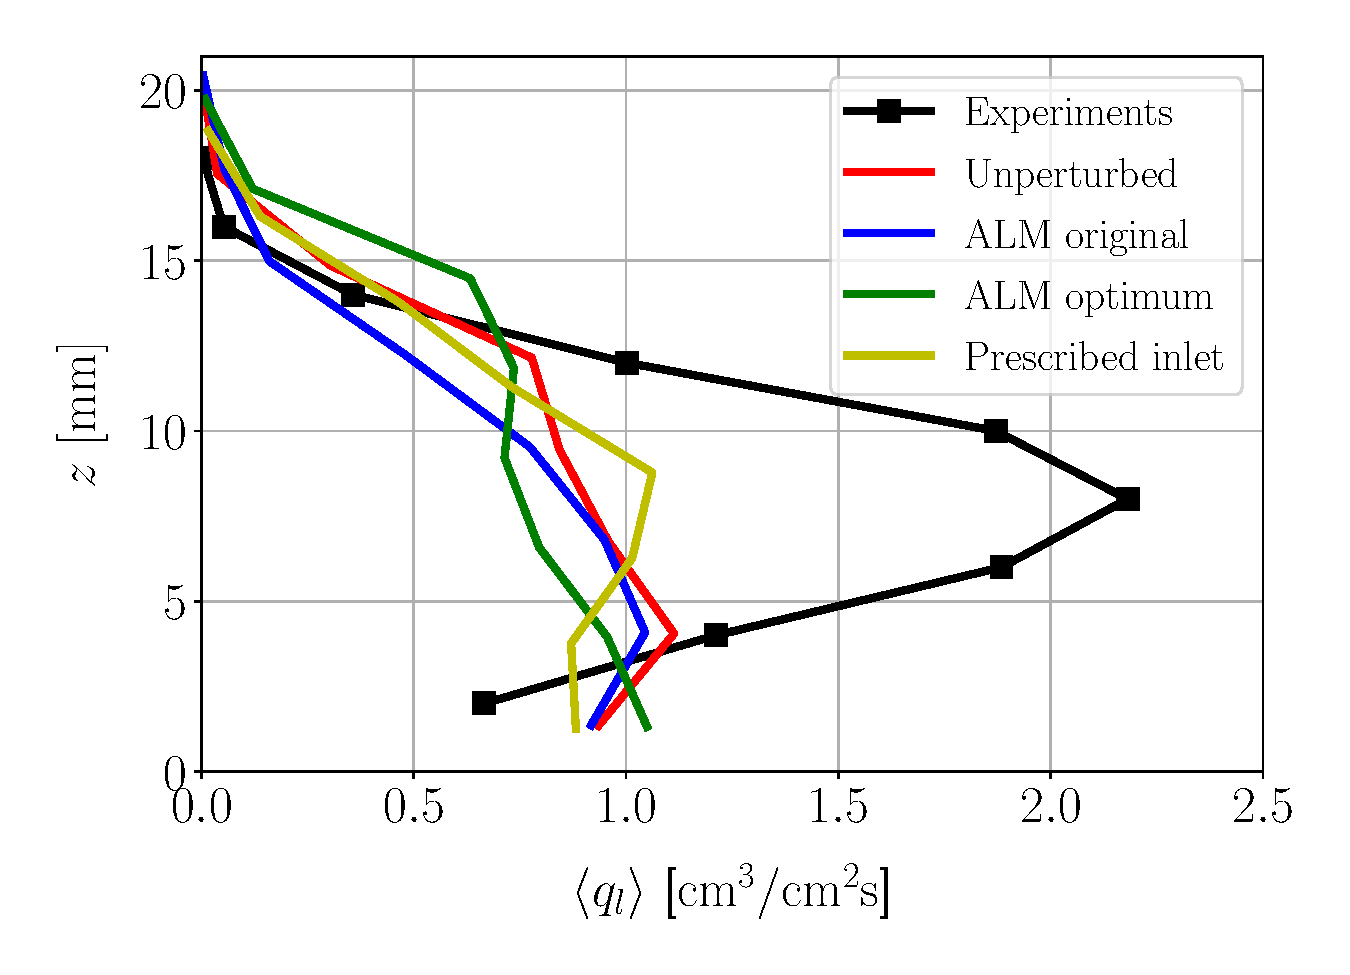
\includegraphics[scale=0.3]{./part2_developments/figures_ch6_lagrangian_JICF/expe_validation_set_1/integrated_fluxes_along_z}
   \hfill
   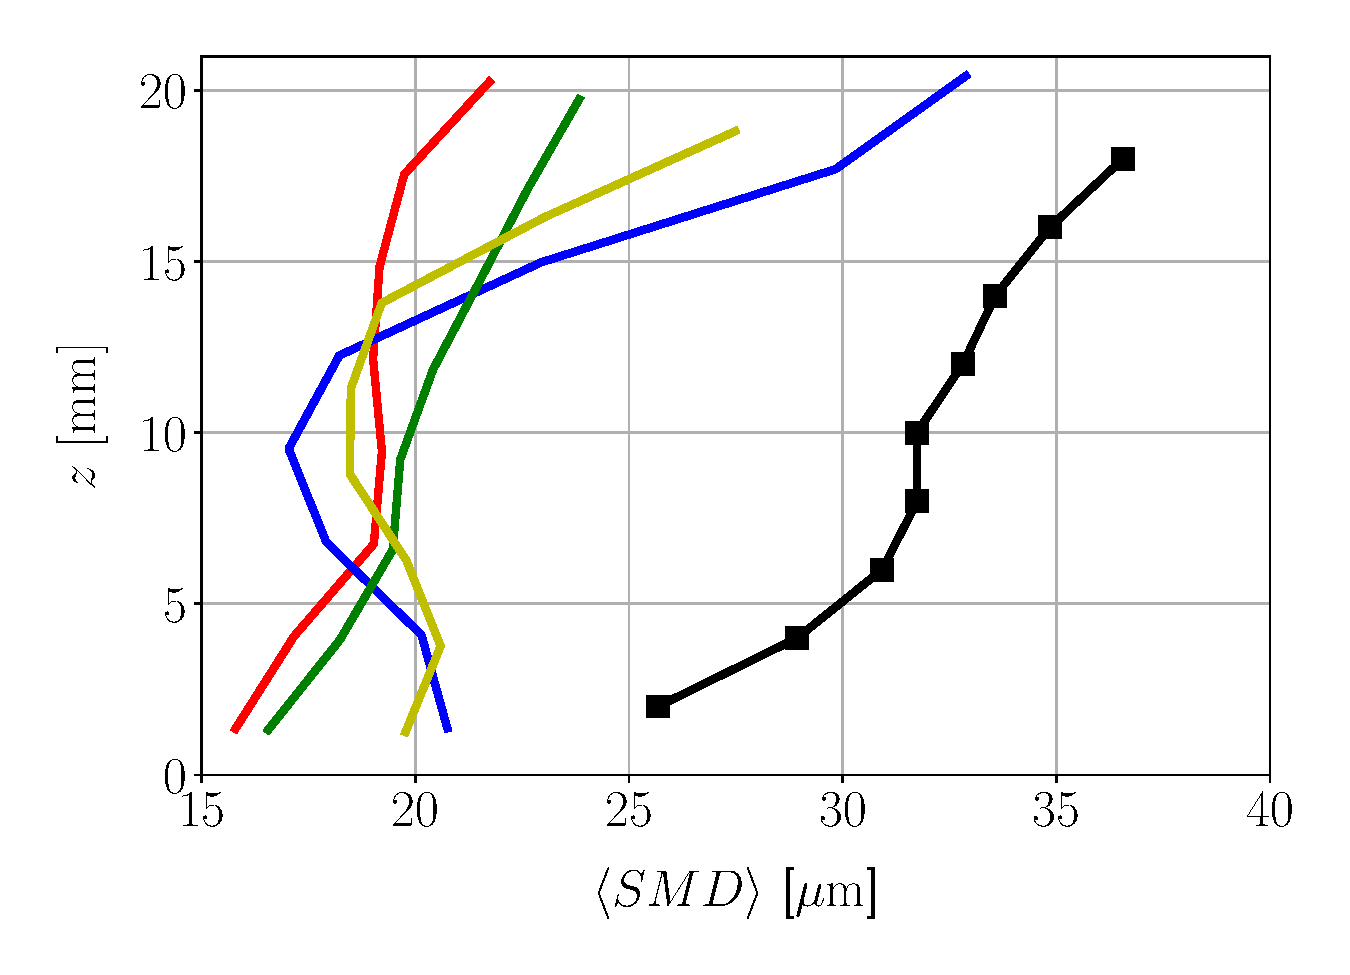
\includegraphics[scale=0.3]{./part2_developments/figures_ch6_lagrangian_JICF/expe_validation_set_1/integrated_SMD_along_z}
	\caption{Magnitudes integrated along the $y$ direction}
\end{subfigure}

\vskip\baselineskip

\begin{subfigure}[b]{0.9\textwidth}
	\flushleft
   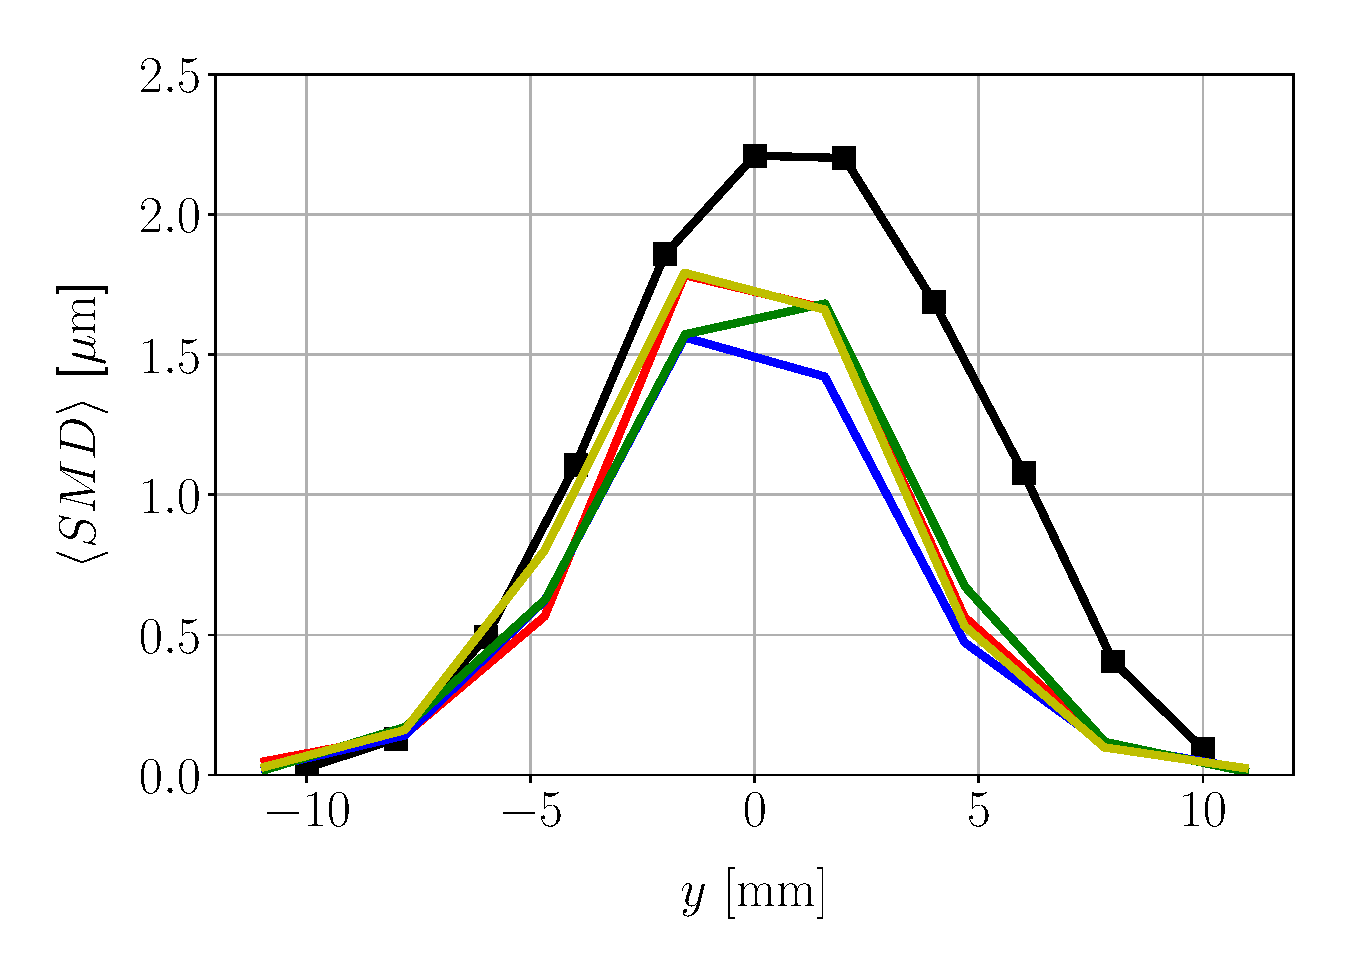
\includegraphics[scale=0.3]{./part2_developments/figures_ch6_lagrangian_JICF/expe_validation_set_1/integrated_fluxes_along_y}
   \hfill
   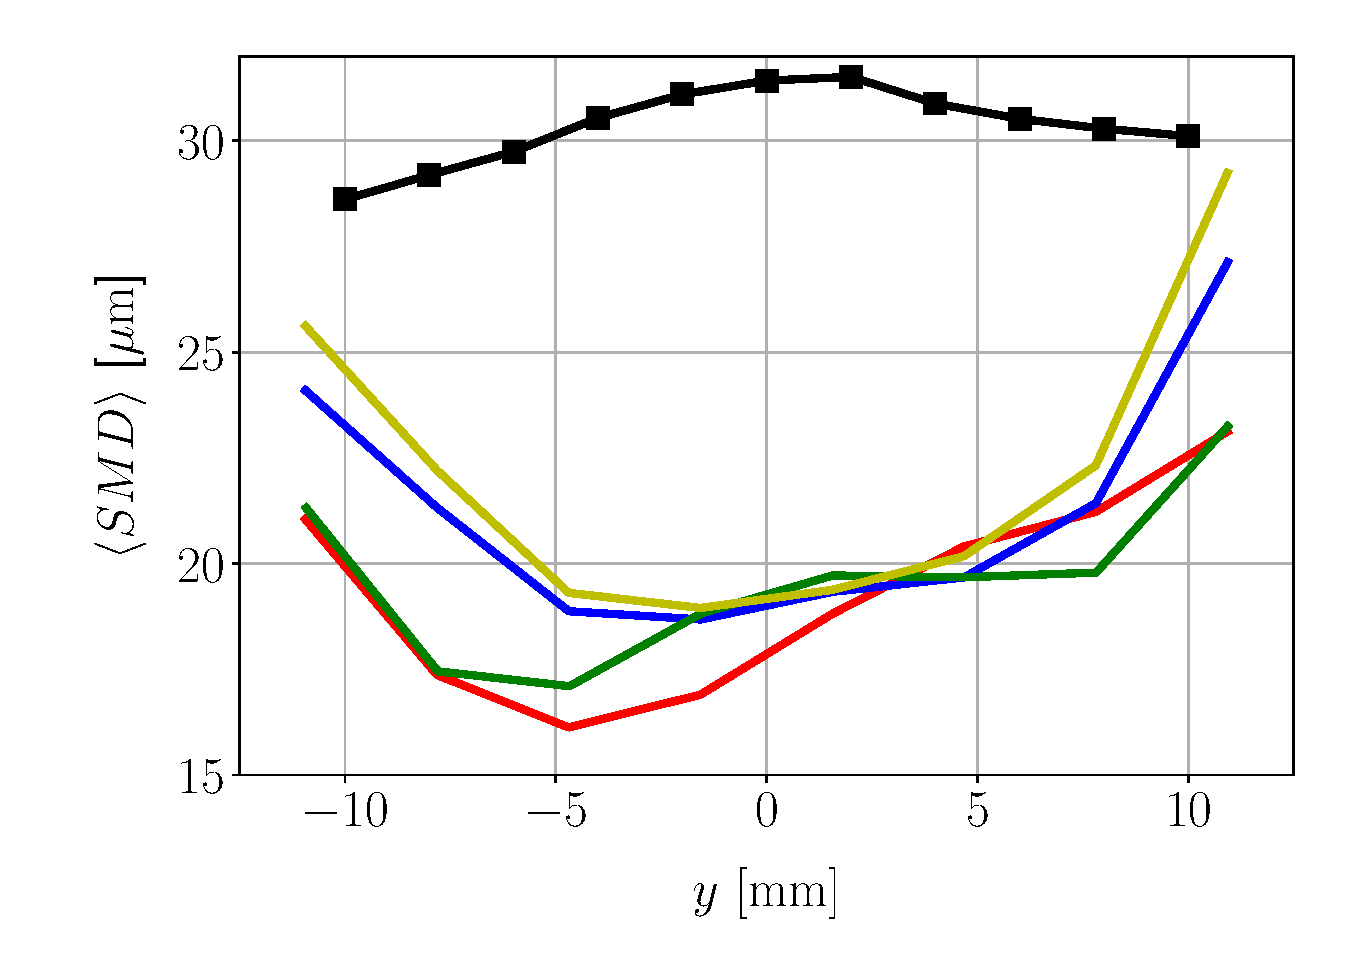
\includegraphics[scale=0.3]{./part2_developments/figures_ch6_lagrangian_JICF/expe_validation_set_1/integrated_SMD_along_y}
	\caption{Magnitudes integrated along the $z$ direction}
\end{subfigure}

   \caption{Set I: Integrated $SMD$ and $q_l$ values at $x = 80$ mm and comparison with experimental results}
%\label{fig:jicf_liquid_mean_velocities_with_x}
\end{figure}


\subsection{Set II: influence of SLI parameters}

\subsection{Set III: influence of secondary atomization model}

\subsection{Set IV: influence of resolved parameters}

\begin{table}[!h]
\centering
\caption{SMD values at $x = 80$ mm for simulations from Set I}
\begin{tabular}{ccc}
\thickhline
Case & $SMD~\left[\mu \mathrm{m} \right]$ & $\varepsilon_{SMD}~\left[\% \right]$ \\
\thickhline
Experiments high We & 31 & - \\
IV.1 - $x_\mathrm{inj} = 10$ mm & \hl{?} & \hl{?} \\
I.2 - $\Delta x_\mathrm{min} = 20~\mu$m & \hl{?} & \hl{?} \\
I.3 - No turbulence & \hl{?} & \hl{?} \\
\hline 
Experiments low We & 36 & - \\
I.4 - Low Weber point & 27 & - 25 \\
\thickhline
\end{tabular}
\label{tab:results_set_4}
\end{table}

\subsubsection{IV.4 - Operating point}

\begin{figure}[ht]
\flushleft
\begin{subfigure}[b]{0.9\textwidth}
	\flushleft
   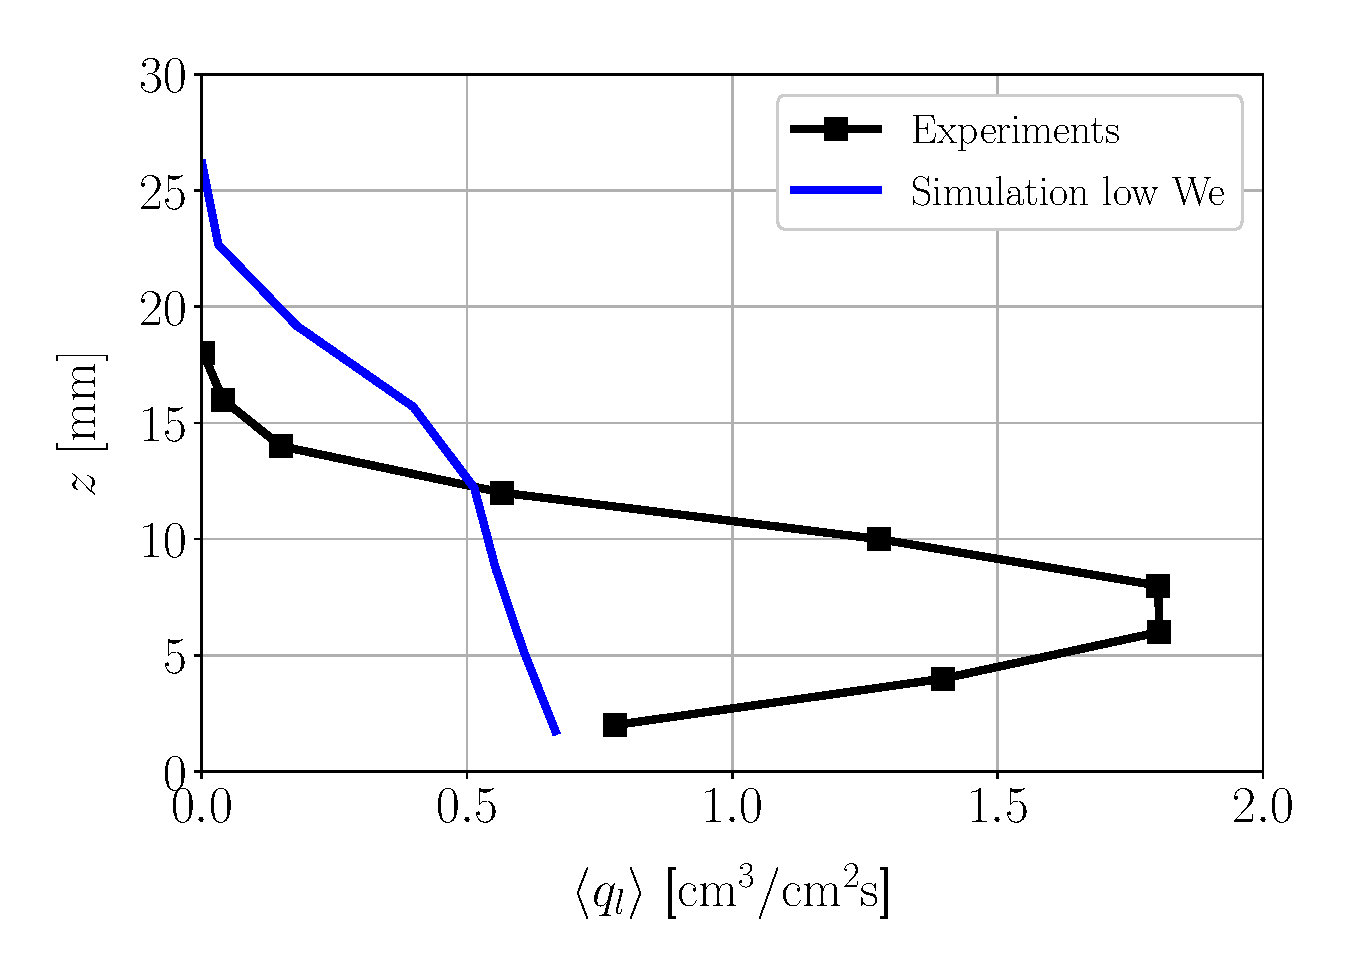
\includegraphics[scale=0.3]{./part2_developments/figures_ch6_lagrangian_JICF/expe_validation_set_4/integrated_fluxes_along_z}
   \hfill
   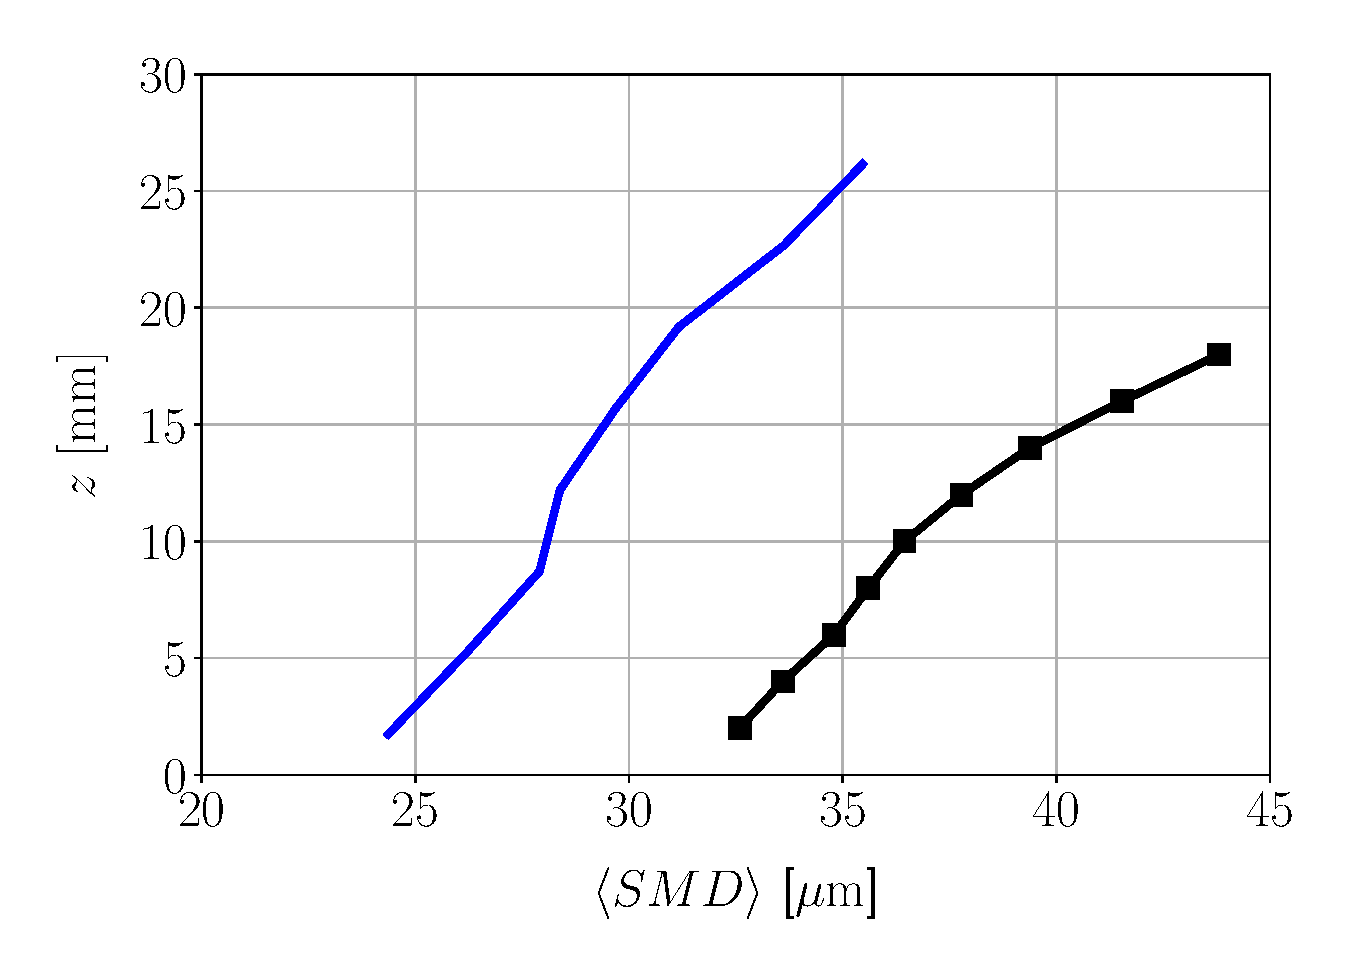
\includegraphics[scale=0.3]{./part2_developments/figures_ch6_lagrangian_JICF/expe_validation_set_4/integrated_SMD_along_z}
	\caption{Magnitudes integrated along the $y$ direction}
\end{subfigure}

\vskip\baselineskip

\begin{subfigure}[b]{0.9\textwidth}
	\flushleft
   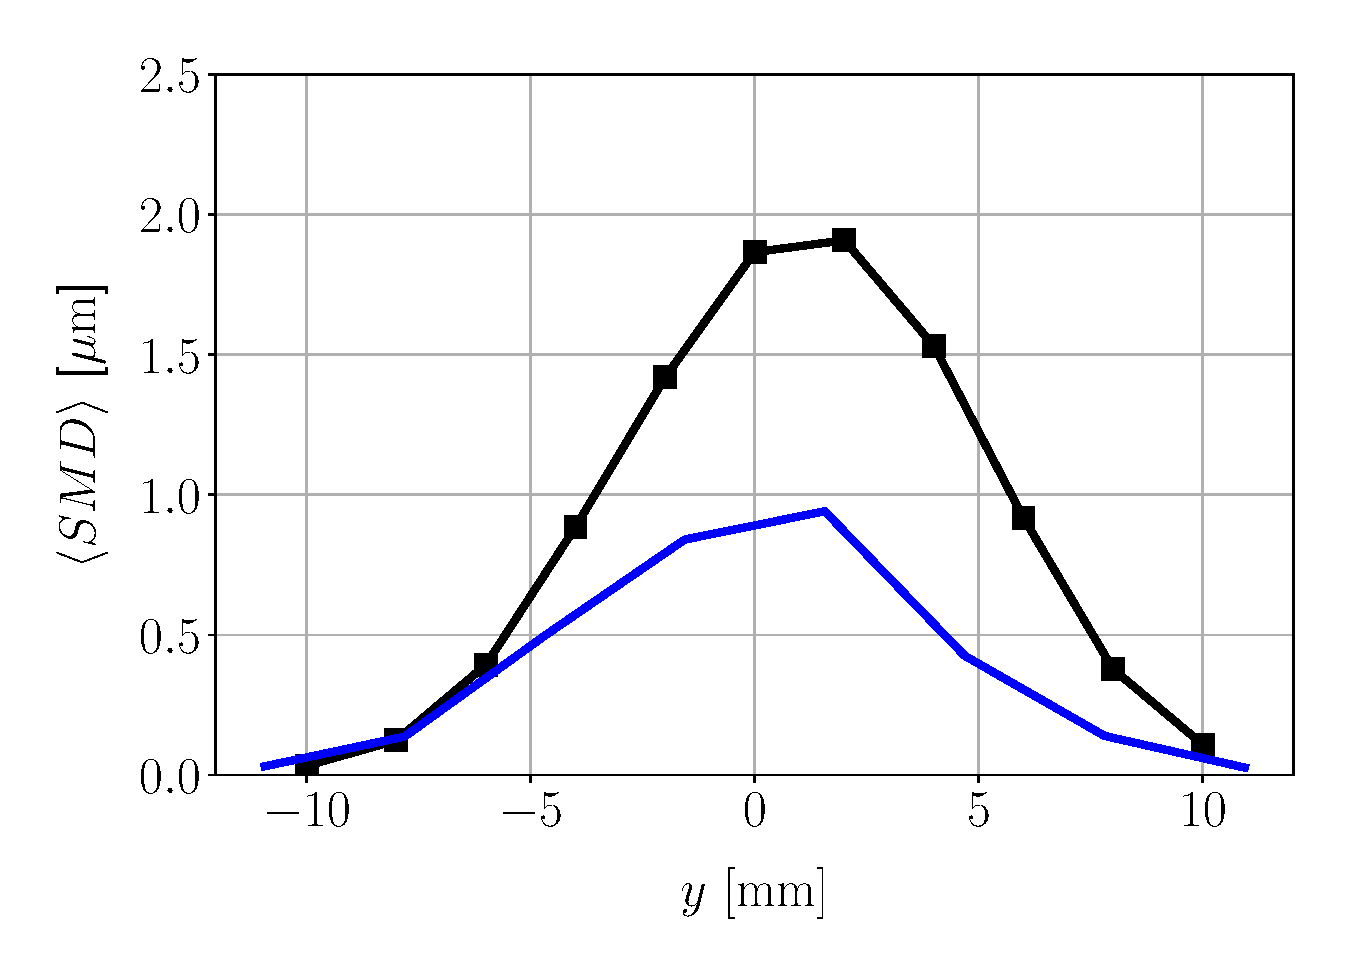
\includegraphics[scale=0.3]{./part2_developments/figures_ch6_lagrangian_JICF/expe_validation_set_4/integrated_fluxes_along_y}
   \hfill
   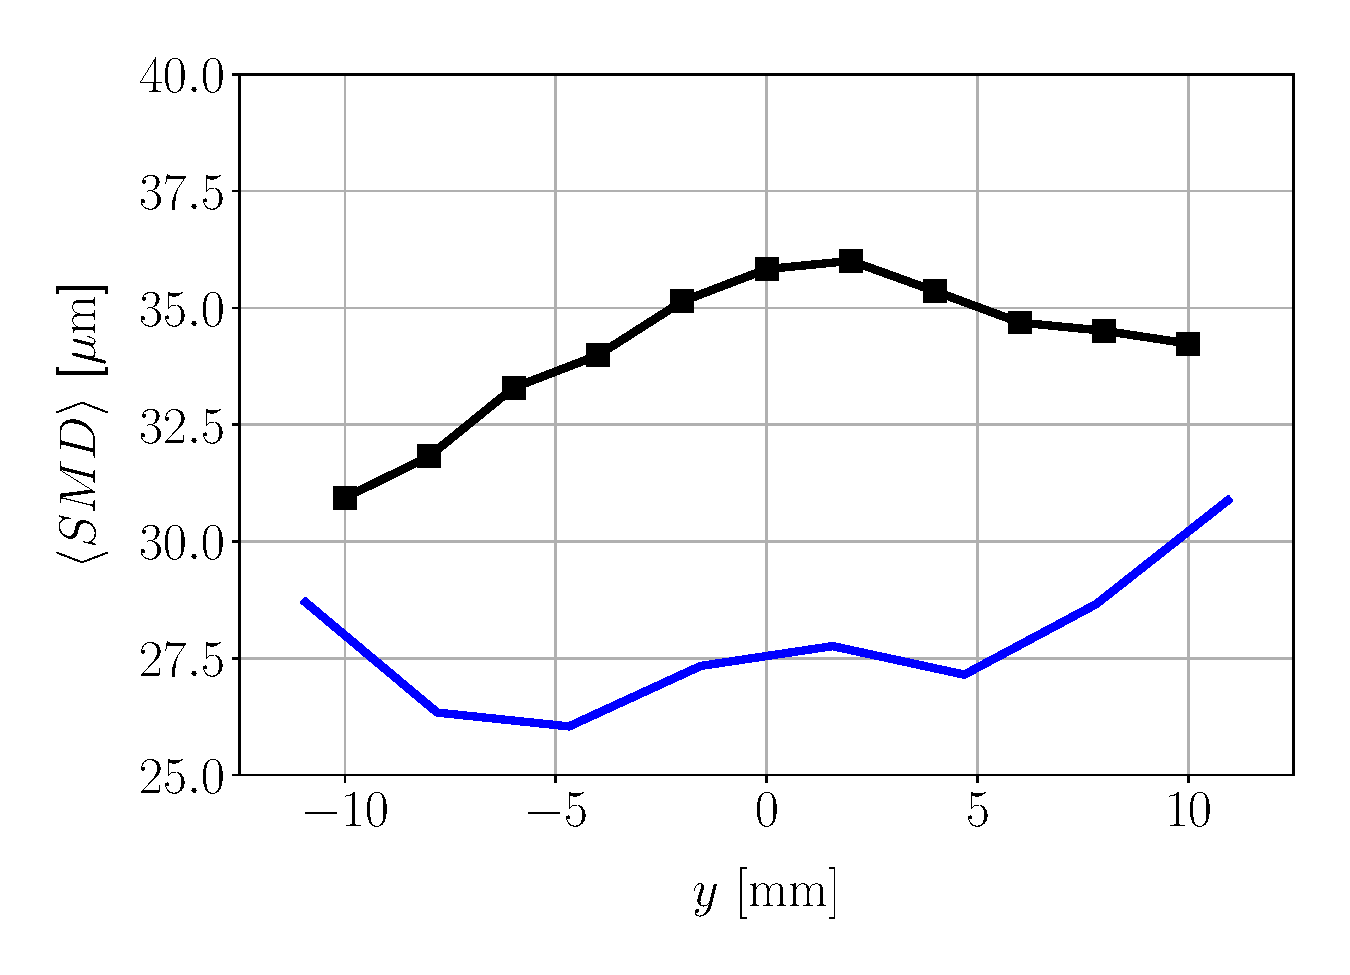
\includegraphics[scale=0.3]{./part2_developments/figures_ch6_lagrangian_JICF/expe_validation_set_4/integrated_SMD_along_y}
	\caption{Magnitudes integrated along the $z$ direction}
\end{subfigure}

   \caption{Set IV, effect of operating condition: Integrated $SMD$ and $q_l$ values at $x = 80$ mm and comparison with experimental results}
%\label{fig:jicf_liquid_mean_velocities_with_x}
\end{figure}



\clearpage

\section{Additional considerations}

\subsection{Lagrangian trajectories}

\subsection{Frequential analysis}

\section{Conclusions}

\section{Relation between volume and mixture fractions}

So we can relate $\overline{\alpha}$ field with the mixture fraction somehow, this will be interesting for people doing combustion. I have developed the following relation between mixture fraction $Z$ and volume fraction $\alpha$ (need to check it properly):

\begin{equation}
Z = \frac{m_l}{m_l + m_g} = \frac{V_l \rho_l}{V_l \rho_l + V_g \rho_g} = \frac{1}{1 + \frac{V_g}{V_l} \frac{\rho_g}{\rho_l}} = \frac{1}{1 + \frac{\rho_g}{\rho_l} \frac{1 - \alpha}{\alpha}}
\end{equation}


We can also make a link to heat relase, for the interest of combustion studies.




\section{Results}

%\subsection{Mesh convergence study}

\subsection{Validation with experiments (quantitative/qualitative)}

\subsection{Trajectories}

In order to illustrate the lagrangian trajectories and the continuity with respect to the resolved jets, a volume fraction field can be defined in the lagrangian simulations:

\begin{equation}
\alpha_l \left( \textbf{x}, t \right) = \frac{V_l \left( \textbf{x}, t \right)}{V_{el}}
\end{equation}

where $V_{el}$ is the volume of the element in the eulerian mesh grid. Therefore, the volume fraction is a magnitude defined in the main eulerian grid. Since the dispersed phase is not directly represented in this grid but by lagrangian particles, $V_l \left( \textbf{x}, t \right)$ is calculated by interpolating the volume of the particles located within each element at each iteration.

\subsection{Frequential analysis}

Several probes have been located in the outer part of the jet to see the spectra. See Figures \ref{fig:probes_dx10m} and \ref{fig:probes_dx20m} for volume fraction probes, and Figure \ref{fig:probes_U_planey0} for determining velocity spectra at plane y = 0. These are available at pilotage 30-04-2021.

Para velocidades: OJITO con la probe 18 !

\begin{figure}[h!]
	\centering
	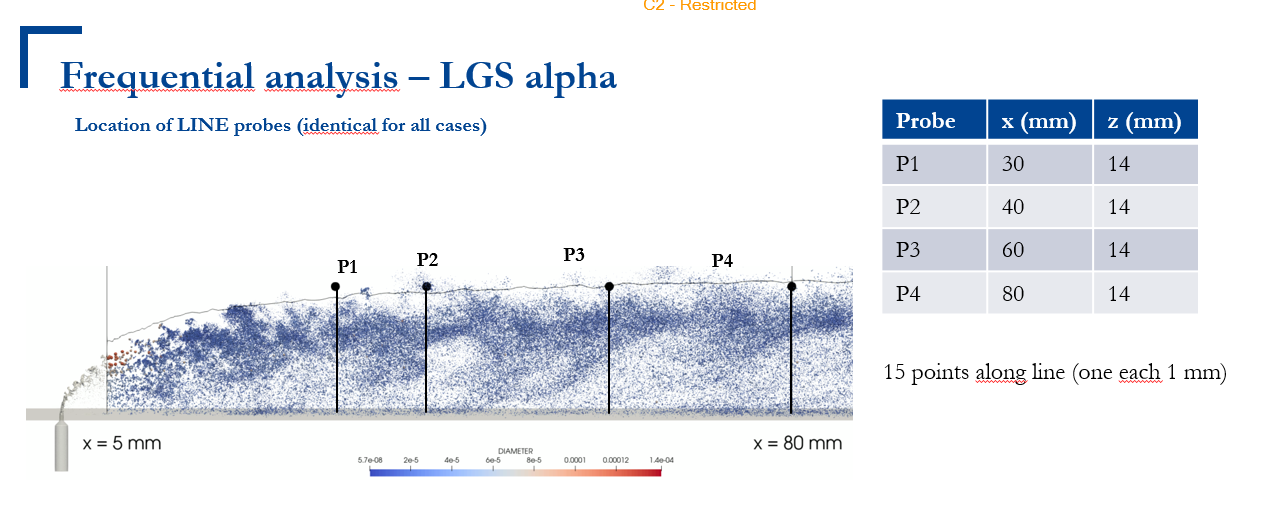
\includegraphics[scale=0.7]{./part2_developments/figures_ch6_lagrangian_JICF/probes_vol_frac}
	\caption{Probes for $\alpha$ frequential analysis for volume fraction}
	\label{fig:probes_dx10m}
\end{figure}


\begin{figure}[h!]
	\centering
	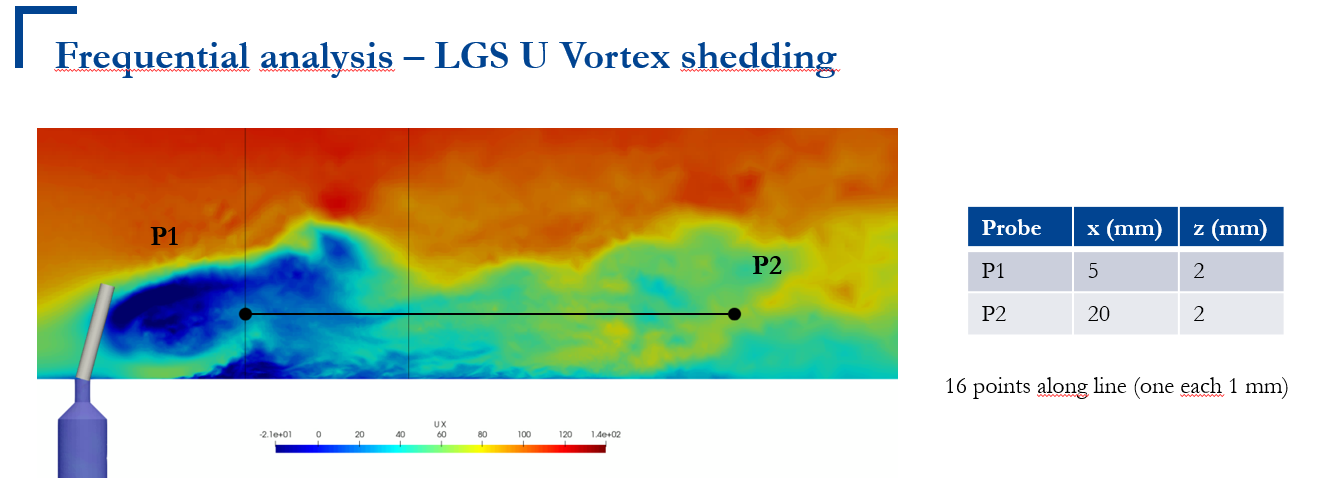
\includegraphics[scale=0.7]{./part2_developments/figures_ch6_lagrangian_JICF/probes_U_planey0}
	\caption{Probes for $U$ study}
	\label{fig:probes_U_planey0}
\end{figure}

\section{Performance of the simulations}

These ones are cheaper than the resolved ones.



\section{Conclusions}

\clearpage

\section{Equations}

	
\begin{equation}
r_\mathrm{crit} = \frac{We_\mathrm{crit} \sigma}{\rho_g u_\mathrm{rel,SPS}^2}
\end{equation}
	
\begin{equation}
t_{bu} = B \sqrt{\frac{\rho_l}{\rho_g}} \frac{r}{u_{rel,SPS}}
\end{equation}

\subsection{Lognormal law actuator}

\begin{subequations}
\label{eq:ALM_SLI_lift_drag_definitions}
\begin{align}
L \left( s_p \right) &= - |\textbf{F}_z \left( s_p \right) | \cos \theta  \\
D \left( s_p \right) &= |\textbf{F}_x \left( s_p \right) | \sin \theta 
\end{align}
\end{subequations}

\begin{equation}
|\textbf{F}_x \left( s_p \right) |  = |\textbf{F}_\mathrm{DC}| \frac{f \left( s_p, \mu_x, \sigma_x \right) s_p}{\sum_{p=1}^{N_p} f \left( s_p, \mu_x, \sigma_x \right) s_p}
\end{equation}

\begin{equation}
|\textbf{F}_z \left( s_p \right) |  = |\textbf{F}_\mathrm{DC}| \frac{f \left( s_p, \mu_z, \sigma_z \right) s_p}{\sum_{p=1}^{N_p} f \left( s_p, \mu_z, \sigma_z \right) s_p}
\end{equation}

\begin{equation}
 f \left( s_p, \mu, \sigma \right) = \frac{1}{s_p \sigma \sqrt{2 \pi }} \exp \left[ - \frac{ \left( \ln s_p - \mu \right)^2}{2 \sigma^2} \right]
\end{equation}

	
\subsection*{Flux stuff}

\begin{equation}
Q_{l,i,j} =  q_{l,i,j} \cdot S_\mathrm{probe}
\end{equation}

\begin{equation}
Q_{l,\mathrm{total}} = \sum_{i=1}^{Ny} \sum_{j=1}^{Nz} Q_{l,i,j} = 4061.5~mm^3/s
\end{equation}

\begin{equation}
Q_{l,\mathrm{injected}} = \frac{\pi}{4} d_\mathrm{inj}^2 u_l = 3710~mm^3/s
\end{equation}

\begin{equation}
u_l
\end{equation}

\begin{equation}
\epsilon = \frac{|\overline{\textbf{u}}_\mathrm{rel,LGS}| - |\overline{\textbf{u}}_\mathrm{rel,SPS}|}{|\overline{\textbf{u}}_\mathrm{rel,SPS}|}
\end{equation}